% Parlare del tipo di robot, diff drive, ecc. (?)

\chapter{Working in a real environment}
\label{cha:realworld}

The first thing we need is the robot: this projects uses the one shown in \autoref{fig:shelfino}, and it comes from \acrfull{disi} of University of Trento.

\bigskip

\begin{figure}[h]
  \centering
  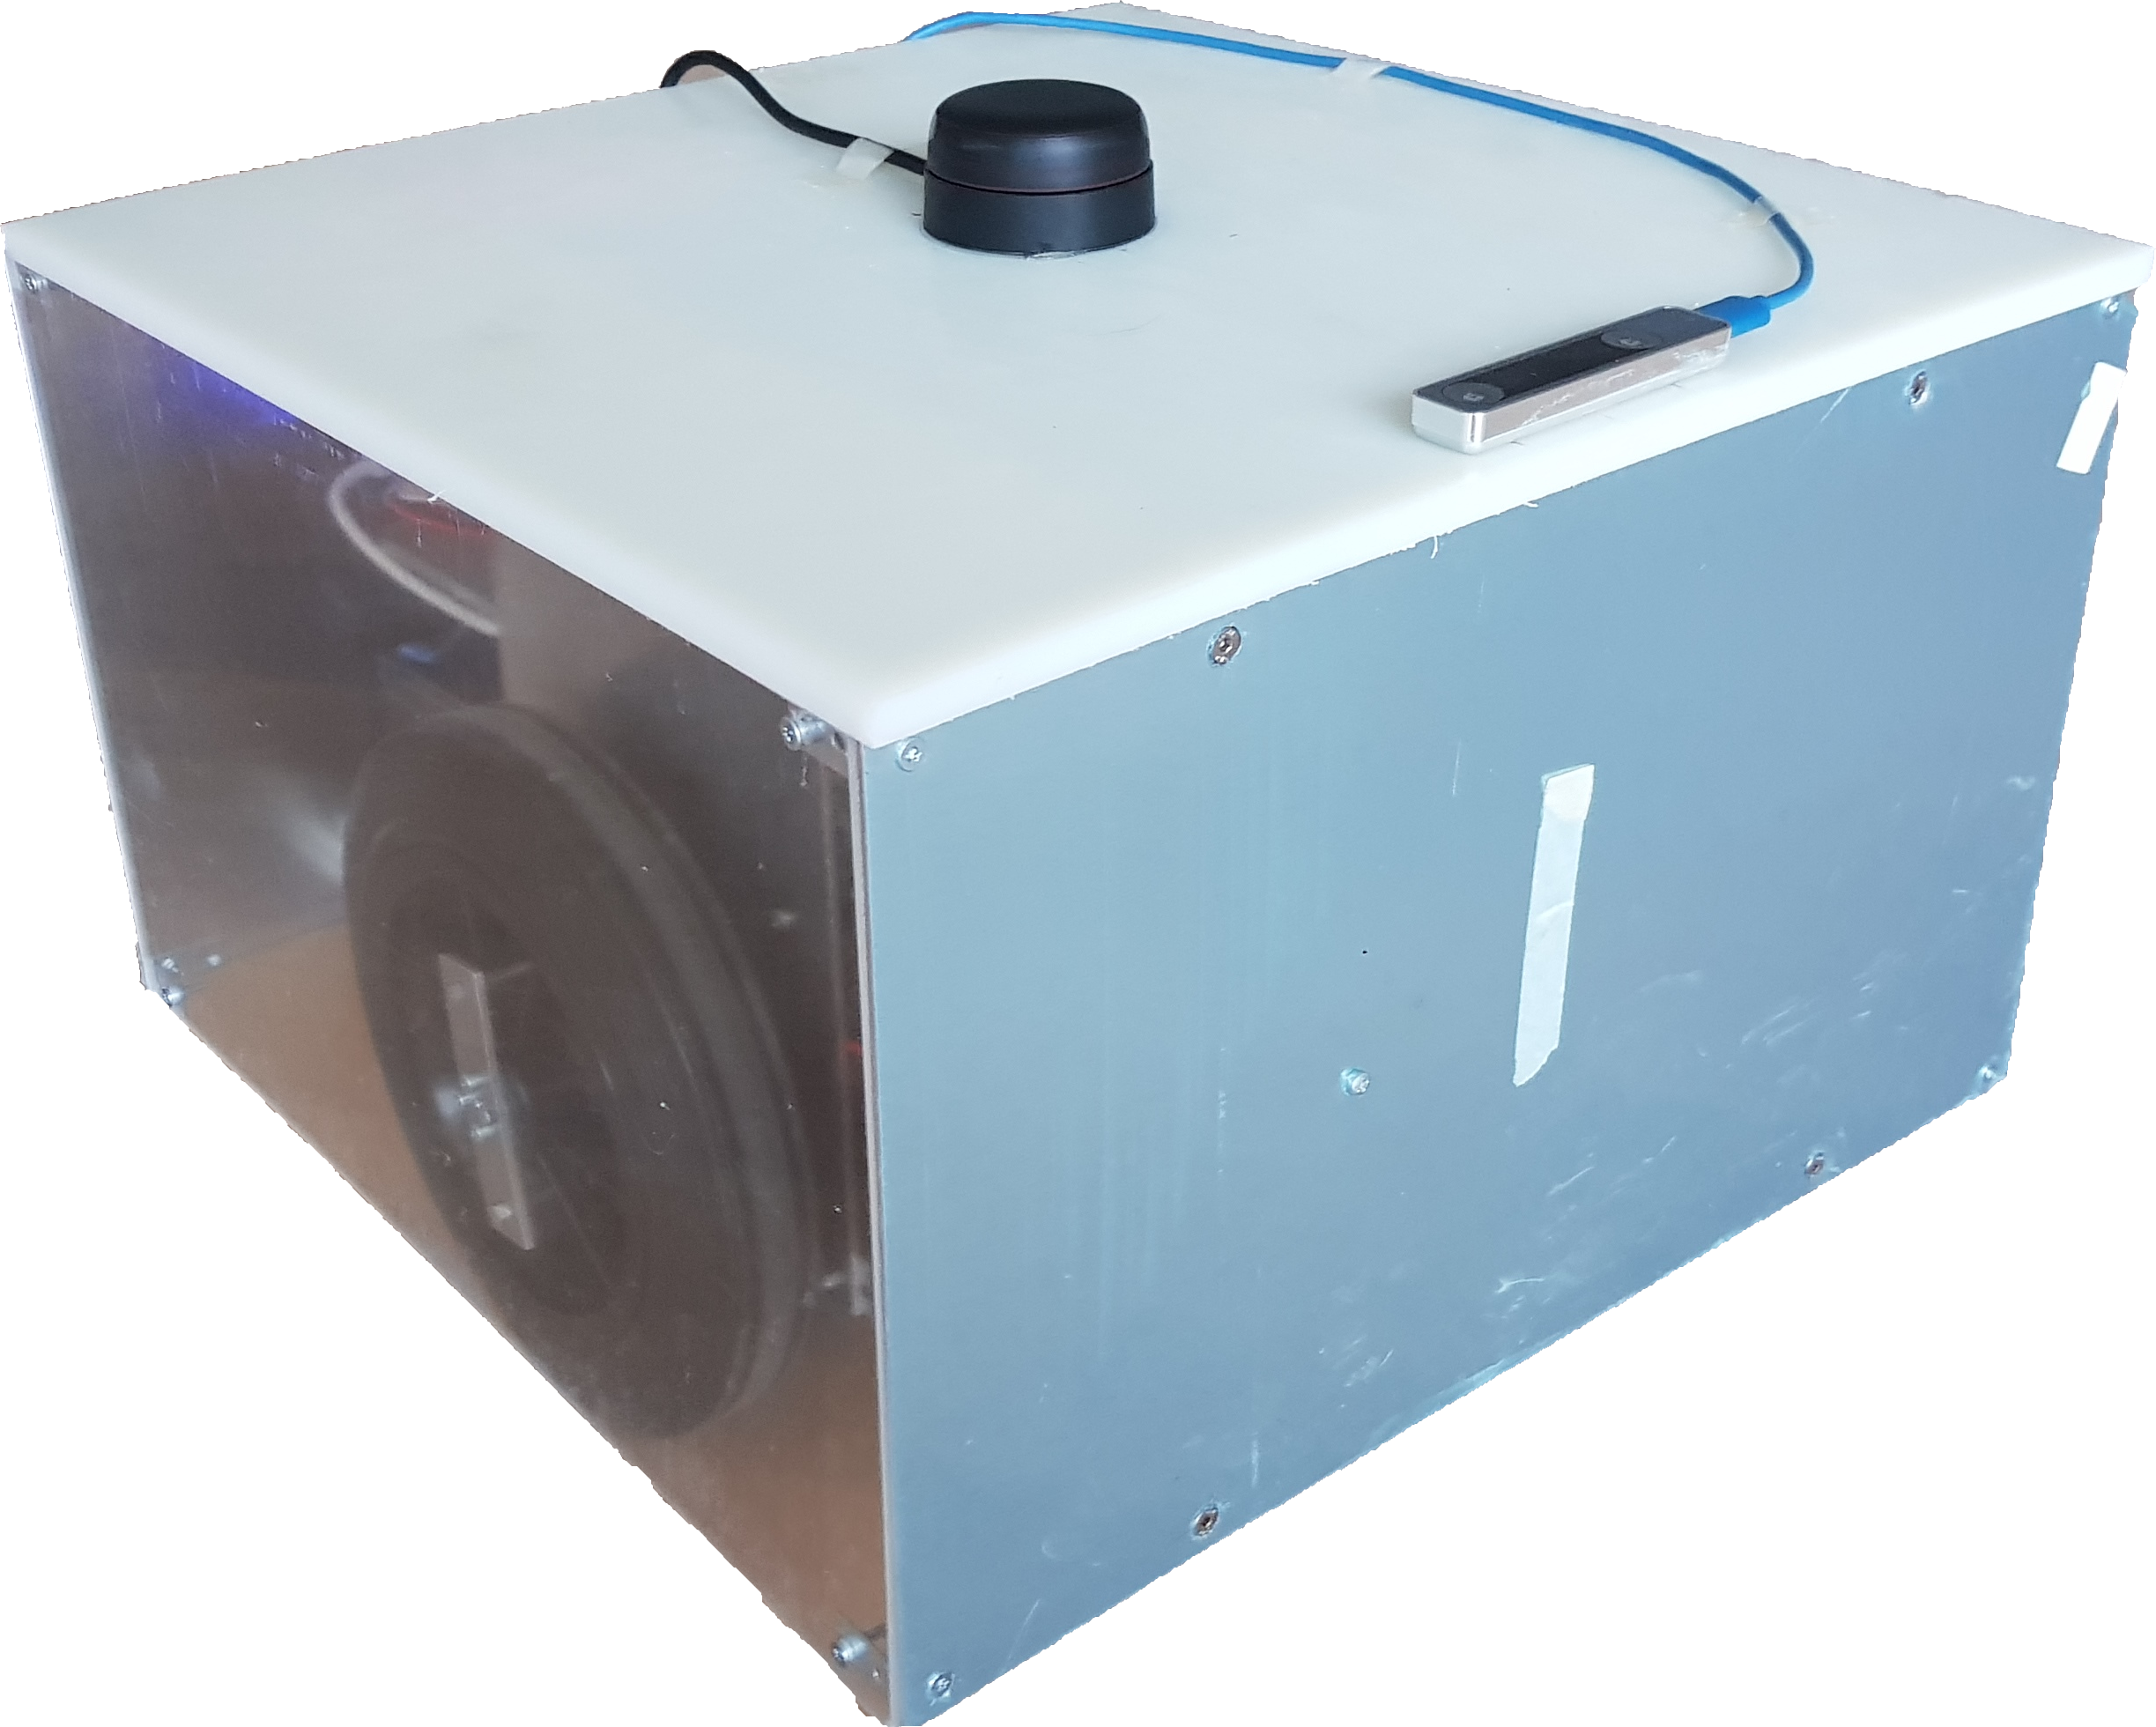
\includegraphics[width=0.5\textwidth]{images/shelfino}
  \caption{The, so called, \textit{shelfino (one)} robot}
  \label{fig:shelfino}
\end{figure}

\section{Shelfino setup} 

\subsection{Adapting existing code}

The \textbf{hardware interface} had already been developed by some researchers in recent years, and they are now no longer here. The original idea was to develop some ROS nodes that would connect to \textbf{encoders}, \textbf{motors drivers} and \textbf{lidars}, but I was not given specific information about brands or manufacturers of some of these components.

Another attempt was to rewrite the code in ROS2: it was not straightforward, and in the end it did not work, since the libraries used refer to a network infrastructure that I am not well aware of. In addition, some features have not been ported to \acrshort{ros}2 \textbf{in the same way}, leading to some potential \textbf{differences} from the original code.

\subsection{\acrshort{ros}1 Bridge}

The final attempt involved the use of a \acrshort{ros}2 package called \textit{ros1\_bridge}. Because both \acrshort{ros}1 and \acrshort{ros}2 use their \textbf{local network} to deliver messages, you can create a node that \textbf{listens to both networks} and when something is received from one side, it is sent to the other: this way you can run the \textbf{existing code as it is} on a \acrshort{ros}1 node (with its dependencies), while making use of its topics and services on a \acrshort{ros}2 workspace at the same time.

But, in order to run both \acrshort{ros}1 and \acrshort{ros}2 nodes on the same machine (or Docker container), they need the same version of Ubuntu. \textbf{\acrshort{ros}2 Foxy} version is mandatory due to planning libraries, and runs only on \textbf{Ubuntu 20.04}, so also \acrshort{ros}1 must use it; the original code, however, was written for the previous version (\acrshort{ros}1 Melodic, running only on Ubuntu 18.04), but furtunately it works smoothly on the new one\footnote{The biggest change was introducing the support for Python 3}, \textbf{\acrshort{ros}1 Noetic} (for the same version of the \acrshort{os}).

To be more precise, the \code{dynamic\_bridge} of this package was used, instead of \code{parametric\_bridge} and \code{static\_bridge}: with the first one you can choose what topics or services you want to bridge, but it has some bugs and does not work well, while the second one must be compiled whenever there are some changes; the dynamic one, instead, adapts to every occasion.

\subsection{Existing nodes explained}
\label{subsec:nodes}

In order to start the existing nodes, a custom launch file was created. A launch file is a file containing information about \textbf{which nodes}, possibly with some \textbf{parameters}, must be \textbf{started} when the system is launched, instead of doing it one by one. Three nodes are inside this launch file:

\begin{itemize}
    \item \code{lidar\_position}
    \item \code{hw\_interface}
    \item \code{odom\_node}
\end{itemize}

\subsubsection{lidar\_position} % forse togliere e forse  mettere 0.43 (?), dire che è stata fatta su ros2 ora

\begin{lstlisting}[
  label={lst:lidarpos},
  language=xml,
  style=xmlStyle
  ]
  <node pkg="tf" type="static_transform_publisher" name="lidar_position"
    args="0 0 0.45 0 0 0 base_link base_laser 10" />
\end{lstlisting}

This is a node (with a custom name) of the \acrshort{ros}1 \code{tf} package, \textit{a package that lets the user keep track of multiple coordinate frames over time [...] and lets the user transform points, vectors, etc. between any two coordinate frames at any desired point in time}.\cite{tf} The node executable is called \code{static\_transform\_publisher} and it is used to \textit{publish a static coordinate transform to tf using an x/y/z offset in meters and roll/pitch/yaw in radians [...]. The period, in milliseconds, specifies how often to send a transform}. \cite{tf} 
As \autoref{lst:lidarpos} shows, here it is used to describe the \textbf{transformation} between \code{base\_link}, that is the root frame (located on the ground under the robot, in the origin), and \code{lidar\_link} (0.45 meters above) every \code{10ms}. So when some points are returned by the laser scans, we also know the height, not otherwise specified, since it is a 2D scan.

\subsubsection{hw\_interface}

It is a node designed to interface with the \textbf{underlying hardware}, thanks to the custom \code{hardwareglo\-balinterface} library previously developed by researchers. It is a \textbf{helper class} that uses a \textbf{ZeroMQ framework} to send messages between the hardware (client) and the server running on the BeagleBone, which keeps track of the data received and makes them accessible using class methods.

Basically, using the interface just described, it reads data from \textbf{encoders}, \textbf{lidar} and \textbf{tracking camera} and makes them available as \acrshort{ros}2 topics (\code{/encoders, /scan, /t265}). It also subscribes to a \code{/cmd\_vel} topic from which it reads the desired \textbf{linear} and \textbf{angular velocities} and dispatches them to the robot's motors accordingly.

\subsubsection{odom\_node}

This node uses information received from \textbf{encoders topic} about wheel rotation and \textbf{tracking camera topic}\footnote{A tracking camera is used in addition to wheel rotation to prevent odometry drift. If you do not use a tracking camera, when the robot is facing a wall and the wheels continue to rotate (obviously the robot will not move), odometry will tell the opposite, that it is still moving. When using it, if the robot moves, certainly what the tracking camera perceives changes, otherwise it will not, and it can be used to avoid the above.} to calculate the \textbf{odometry}, which represents an estimate of the \textbf{position} and \textbf{rotation} of the robot from which it started. This new information is then published both as a message in a topic, and as a transformation between \code{odom\_frame} and \code{base\_link}, employed by the \textbf{navigation system} as described in \autoref{cha:navigation}.